% TrustedNutraProducts ProstaPrime Health Guide
% Complete Men's Prostate Health Guide

\documentclass[11pt,oneside,openany]{book}
\usepackage[margin=1in]{geometry}
\usepackage{titlesec}
\usepackage{graphicx}
\usepackage{array}
\usepackage{enumitem}
\usepackage{hyperref}
\usepackage{xcolor}
\usepackage{setspace}

\definecolor{brandblue}{HTML}{1565C0}

\titleformat{\chapter}{\Huge\bfseries\color{brandblue}}{}{0pt}{}
\titleformat{\section}{\Large\bfseries}{}{0pt}{}

\setlength{\parindent}{0pt}
\onehalfspacing

\begin{document}

% ---------- COVER (MUST BE FIRST) ----------
\pagestyle{empty}
\pagenumbering{gobble}

\begin{titlepage}
\newgeometry{margin=0pt}

\noindent
\makebox[\paperwidth][c]{%
  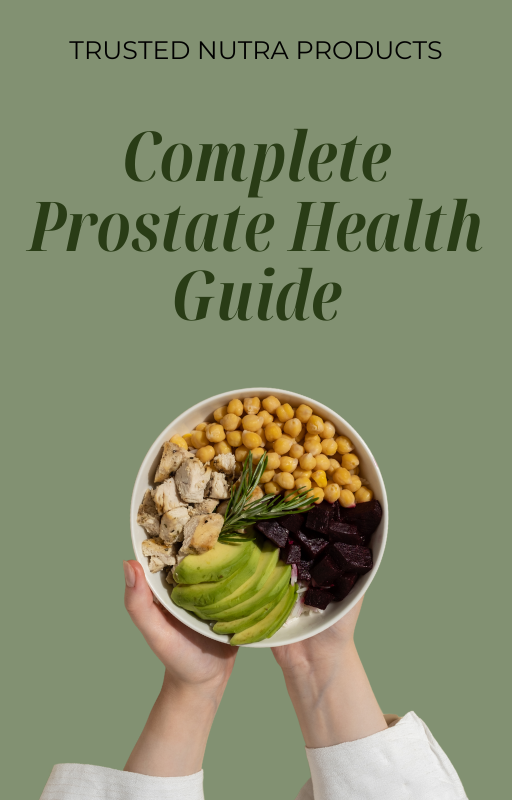
\includegraphics[
    width=\paperwidth,
    height=\paperheight
  ]{ebook1.png}%
}

\end{titlepage}

\restoregeometry
\clearpage
% ---------- END COVER ----------


\pagenumbering{arabic}
\setcounter{page}{1}
\onehalfspacing



%------------------ INTRODUCTION ------------------

\chapter*{Welcome to Better Prostate Health}
\addcontentsline{toc}{chapter}{Welcome to Better Prostate Health}

This isn't just another generic health guide. This is made specifically for men who refuse to accept declining vitality, frequent nighttime bathroom trips, and weakening bladder control as "just part of getting older."

The truth? Your prostate health is directly connected to your energy, confidence, and quality of life. And you have more control than you think.

\section*{What You'll Discover}
\begin{itemize}[leftmargin=*]
\item The prostate-testosterone connection nobody talks about
\item Why most men are deficient in the TWO minerals critical for prostate health
\item 10 warning signs that demand immediate action
\item Power foods that reduce inflammation and support healthy function
\item Environmental toxins secretly disrupting your hormones
\item Simple daily habits that restore bladder control
\item How ProstaPrime accelerates natural recovery
\end{itemize}

\section*{This Guide Is For You If:}
\begin{itemize}[leftmargin=*]
\item You're tired of waking up 2--4 times per night to urinate
\item You want to reclaim your energy and confidence
\item You're ready to take control with science-backed strategies
\item You refuse to accept "it's just your age" as an answer
\end{itemize}

\textbf{Fair Warning:} This guide requires action. Reading won't fix anything. Implementation will.

\clearpage
\tableofcontents

\clearpage
%------------------ CHAPTER 1 ------------------

\chapter*{Understanding Your Prostate \& Bladder}
\addcontentsline{toc}{chapter}{Understanding Your Prostate \& Bladder}

\section*{What Is the Prostate?}

The prostate is a small walnut-sized gland located below the bladder. It surrounds the urethra and plays a key role in male reproductive health by producing fluid that nourishes and transports sperm.

\textbf{Key Functions:}
\begin{itemize}[leftmargin=*]
\item Produces seminal fluid
\item Helps control urination
\item Supports fertility
\end{itemize}

\section*{How the Prostate Changes with Age}

As men age, the prostate naturally enlarges. This condition, called benign prostatic hyperplasia (BPH), can press against the urethra and cause urinary symptoms.

\textbf{Common Age-Related Changes:}
\begin{itemize}[leftmargin=*]
\item Gradual enlargement starting around age 40
\item Increased pressure on the bladder
\item More frequent urination, especially at night
\item Difficulty starting or stopping urination
\end{itemize}

\section*{The Prostate-Bladder Connection}

Your prostate and bladder work together. When the prostate enlarges, it can:
\begin{itemize}[leftmargin=*]
\item Restrict urine flow
\item Cause incomplete bladder emptying
\item Lead to urgency and frequency
\item Weaken bladder muscles over time
\end{itemize}

Understanding this connection is the first step toward taking control of your health.

\clearpage
%------------------ CHAPTER 2 ------------------

\chapter*{10 Warning Signs Men Should Never Ignore}
\addcontentsline{toc}{chapter}{10 Warning Signs Men Should Never Ignore}

Pay attention to these symptoms. Early detection and lifestyle changes can make a significant difference.

\section*{1. Frequent Nighttime Urination (Nocturia)}
Waking up 2+ times per night to urinate can disrupt sleep and signal prostate enlargement.

\section*{2. Weak or Interrupted Urine Stream}
Difficulty maintaining a strong, steady flow may indicate urethral obstruction.

\section*{3. Difficulty Starting Urination}
Hesitancy or straining to begin urinating is a common early sign of BPH.

\section*{4. Feeling of Incomplete Bladder Emptying}
If you feel like your bladder isn't fully empty after urination, it's worth investigating.

\section*{5. Sudden, Urgent Need to Urinate}
Urgency that's hard to control can be a sign of bladder irritation or prostate pressure.

\section*{6. Dribbling After Urination}
Post-void dribbling is common but shouldn't be ignored if it worsens.

\section*{7. Blood in Urine or Semen}
This requires immediate medical attention to rule out serious conditions.

\section*{8. Pain or Burning During Urination}
May indicate infection, inflammation, or other prostate issues.

\section*{9. Lower Back or Pelvic Pain}
Chronic discomfort in these areas can be linked to prostate health.

\section*{10. Erectile Dysfunction}
While not always prostate-related, ED can be associated with prostate conditions and should be discussed with a healthcare provider.

\textbf{Important:} If you experience any of these symptoms, consult a healthcare professional. This guide complements, but does not replace, medical advice.

\clearpage
%------------------ CHAPTER 3 ------------------

\chapter*{Power Foods for Prostate Health}
\addcontentsline{toc}{chapter}{Power Foods for Prostate Health}

Here's what most doctors won't tell you: your diet directly impacts your prostate function, hormone balance, and inflammation levels. The right foods act as medicine. The wrong foods accelerate decline.

\section*{The Big Two: Zinc \& Selenium}

\textbf{Zinc} is concentrated in healthy prostate tissue more than any other organ. Low zinc = enlarged prostate and weakened function.

\textbf{Best Sources:}
\begin{itemize}[leftmargin=*]
\item Pumpkin seeds (1/4 cup daily)
\item Oysters (highest zinc content)
\item Grass-fed beef
\item Cashews and almonds
\end{itemize}

\textbf{Selenium} protects prostate cells from oxidative damage.

\textbf{Best Sources:}
\begin{itemize}[leftmargin=*]
\item Brazil nuts (3--4 daily provides 100\%+ daily value)
\item Wild-caught fish
\item Pasture-raised eggs
\end{itemize}

\section*{Lycopene: The Prostate Protector}
Cooked tomatoes release lycopene, a carotenoid shown in studies to support prostate health.

\textbf{How to Maximize:}
\begin{itemize}[leftmargin=*]
\item Cook tomatoes with healthy fats (olive oil)
\item Tomato paste, sauce, and soup
\item Add daily to eggs, chicken, or pasta
\end{itemize}

\section*{Omega-3 Fatty Acids: Inflammation Fighters}
Chronic inflammation destroys prostate health. Omega-3s reverse it.

\textbf{Top Sources:}
\begin{itemize}[leftmargin=*]
\item Wild-caught salmon (2--3x weekly)
\item Sardines and mackerel
\item Grass-fed beef
\item Walnuts and flaxseeds
\end{itemize}

\section*{Cruciferous Vegetables: Hormone Balancers}
Broccoli, cauliflower, and Brussels sprouts contain DIM (diindolylmethane), which helps metabolize excess estrogen---a major factor in prostate enlargement.

\textbf{Action Step:} Eat 1--2 cups daily, steamed or roasted.

\section*{Vitamin D: The Testosterone Booster}
Over 70\% of men are vitamin D deficient. Low vitamin D correlates with:
\begin{itemize}[leftmargin=*]
\item Enlarged prostate
\item Low testosterone
\item Weakened immunity
\end{itemize}

\textbf{Sources:}
\begin{itemize}[leftmargin=*]
\item Sunlight exposure (15--20 minutes daily)
\item Fatty fish (salmon, mackerel)
\item Egg yolks
\item Supplement: 3,000--5,000 IU daily (consult your doctor)
\end{itemize}

\section*{Green Tea: Daily Defense}
Contains catechins and EGCG, compounds studied for prostate protection.

\textbf{Protocol:} 2--3 cups daily, preferably before 2 PM.

\section*{Healthy Fats: Testosterone Building Blocks}
Your body needs dietary fat to produce testosterone. Low-fat diets tank hormone levels.

\textbf{Best Fats:}
\begin{itemize}[leftmargin=*]
\item Avocados
\item Extra virgin olive oil
\item Grass-fed butter
\item Coconut oil
\end{itemize}

\section*{Foods to ELIMINATE}

\textbf{Soy Products:} Contain phytoestrogens that mimic estrogen and disrupt hormones.

\textbf{Processed Meats:} Linked to increased prostate issues.

\textbf{Excessive Alcohol:} Increases estrogen and tanks testosterone.

\textbf{Plastics \& BPA:} Hormone disruptors. Never microwave food in plastic. Use glass or stainless steel.

\textbf{Sugar \& Refined Carbs:} Spike insulin, increase inflammation, promote fat storage around organs.

%------------------ CHAPTER 4 ------------------

\chapter*{Environmental Toxins Destroying Your Prostate}
\addcontentsline{toc}{chapter}{Environmental Toxins Destroying Your Prostate}

You can eat perfectly and still struggle with prostate issues if you're constantly exposed to hormone-disrupting chemicals. These toxins mimic estrogen, suppress testosterone, and directly damage prostate tissue.

\section*{The Plastic Problem}

\textbf{BPA (Bisphenol A)} and similar chemicals leach from plastics into food and drinks, acting as xenoestrogens (fake estrogen).

\textbf{Immediate Actions:}
\begin{itemize}[leftmargin=*]
\item NEVER microwave food in plastic containers
\item Replace plastic water bottles with glass or stainless steel
\item Avoid canned foods with BPA linings (choose glass jars)
\item Don't drink hot beverages from plastic cups
\end{itemize}

\section*{Personal Care Products}

Most shampoos, soaps, and deodorants contain parabens and phthalates---hormone disruptors absorbed through skin.

\textbf{Switch To:}
\begin{itemize}[leftmargin=*]
\item Natural, paraben-free products
\item Aluminum-free deodorant
\item Fragrance-free when possible (fragrances hide chemicals)
\end{itemize}

\section*{Pesticides in Food}

Conventionally grown produce is sprayed with endocrine disruptors.

\textbf{Solution:}
\begin{itemize}[leftmargin=*]
\item Buy organic for the "Dirty Dozen" (strawberries, spinach, apples, etc.)
\item Wash all produce thoroughly
\item Choose grass-fed, pasture-raised animal products
\end{itemize}

\section*{Household Cleaners}

Chemical cleaners release VOCs (volatile organic compounds) that disrupt hormones.

\textbf{Alternatives:}
\begin{itemize}[leftmargin=*]
\item White vinegar + water for surfaces
\item Baking soda for scrubbing
\item Natural cleaning brands
\end{itemize}

\section*{Non-Stick Cookware}

Teflon and non-stick coatings release toxic fumes when heated.

\textbf{Use Instead:}
\begin{itemize}[leftmargin=*]
\item Cast iron
\item Stainless steel
\item Ceramic cookware
\end{itemize}

\textbf{Bottom Line:} Small swaps add up. Reducing toxic load gives your body the environment it needs to heal.

%------------------ CHAPTER 5 ------------------

\chapter*{Lifestyle Habits That Make a Difference}
\addcontentsline{toc}{chapter}{Lifestyle Habits That Make a Difference}

Diet is half the battle. These habits complete the protocol.

\section*{1. Strategic Hydration}
Drinking water randomly all day guarantees nighttime trips.

\textbf{The Protocol:}
\begin{itemize}[leftmargin=*]
\item Front-load hydration: 70\% of water before 3 PM
\item Sip, don't chug (prevents bladder irritation)
\item Stop drinking 2--3 hours before bed
\item Target: 2--3 liters daily
\end{itemize}

\section*{2. Strength Training (Non-Negotiable)}
Cardio is fine, but strength training builds muscle, increases testosterone, and improves insulin sensitivity---all critical for prostate health.

\textbf{Minimum Effective Dose:}
\begin{itemize}[leftmargin=*]
\item 3--4 sessions weekly
\item Focus on compound movements (squats, deadlifts, presses)
\item Progressive overload (gradually increase weight)
\item 30--45 minutes per session
\end{itemize}

\section*{3. Cold Exposure Therapy}
Cold exposure boosts testosterone, improves circulation, and reduces inflammation.

\textbf{How to Start:}
\begin{enumerate}
\item End every shower with 30--60 seconds of cold water
\item Gradually work up to 2--3 minutes
\item Breathe deeply, stay calm
\item Do this daily, preferably in the morning
\end{enumerate}

\textbf{Why It Works:} Cold exposure activates brown fat, improves mitochondrial function, and elevates mood-boosting hormones.

\section*{4. Master Pelvic Floor Strength}
Weak pelvic floor = poor bladder control, dribbling, and incomplete emptying.

\textbf{Kegel Protocol:}
\begin{enumerate}
\item Contract pelvic muscles (like stopping urination mid-stream)
\item Hold 5--10 seconds
\item Relax 5--10 seconds
\item Perform 3 sets of 10--15 reps daily
\item Progress by holding longer, not doing more reps
\end{enumerate}

\textbf{Pro Tip:} Do these while driving, watching TV, or waiting in line.

\section*{5. Kill Chronic Stress}
Stress elevates cortisol. High cortisol suppresses testosterone and worsens inflammation.

\textbf{Stress-Reduction Stack:}
\begin{itemize}[leftmargin=*]
\item Morning sunlight exposure (10--15 minutes)
\item Daily movement (walks in nature)
\item Deep breathing: 4-7-8 technique (inhale 4s, hold 7s, exhale 8s)
\item Limit news and social media
\item Monthly "unplug" day (no phone, no screens)
\end{itemize}

\section*{6. Sleep Like Your Life Depends on It}
Because it does. Poor sleep tanks testosterone by up to 15\% in one week.

\textbf{Sleep Optimization Protocol:}
\begin{itemize}[leftmargin=*]
\item 7--8 hours nightly (non-negotiable)
\item Completely dark room (blackout curtains, cover LEDs)
\item Cool temperature (65--68°F)
\item No screens 1 hour before bed
\item Consistent sleep/wake times (even weekends)
\end{itemize}

\section*{7. Eliminate Bladder Irritants}
Caffeine and alcohol irritate the bladder lining and increase urgency.

\textbf{Action Steps:}
\begin{itemize}[leftmargin=*]
\item Limit caffeine to morning only
\item Cut alcohol to 2--3 drinks maximum per week
\item Avoid spicy foods if they trigger symptoms
\item Never hold urine---go when you feel the urge
\end{itemize}

\section*{8. Sunlight \& Vitamin D}
Sunlight triggers vitamin D production, which directly impacts testosterone and prostate health.

\textbf{Daily Practice:}
\begin{itemize}[leftmargin=*]
\item 15--20 minutes of direct sunlight (no sunscreen initially)
\item Expose arms, chest, and legs when possible
\item Best times: morning or late afternoon
\item Supplement with 3,000--5,000 IU vitamin D3 if sun exposure is limited
\end{itemize}

\section*{9. Quit Smoking (If You Still Are)}
Smoking restricts blood flow, increases inflammation, and directly damages prostate tissue. There's no safe amount.

\section*{10. Move Daily}
Sitting destroys pelvic circulation. Standing and walking improve blood flow to prostate tissue.

\textbf{Minimum:} 8,000--10,000 steps daily + dedicated exercise sessions.

%------------------ CHAPTER 6 ------------------

\chapter*{How ProstaPrime Supports Your Health}
\addcontentsline{toc}{chapter}{How ProstaPrime Supports Your Health}

ProstaPrime is a natural supplement designed to support prostate and bladder health through carefully selected ingredients.

\section*{Key Benefits}
\begin{itemize}[leftmargin=*]
\item Supports healthy urinary flow
\item Reduces nighttime bathroom trips
\item Promotes bladder control
\item Contains natural ingredients backed by research
\end{itemize}

\section*{Recommended Usage}
\begin{itemize}[leftmargin=*]
\item Take as directed on the bottle
\item Use consistently for best results
\item Combine with healthy lifestyle habits
\item Stay hydrated throughout the day
\end{itemize}

\section*{What Makes ProstaPrime Different}
\begin{itemize}[leftmargin=*]
\item Natural, research-backed ingredients
\item No harsh chemicals or fillers
\item Manufactured in the USA
\item Third-party tested for quality
\end{itemize}

\section*{When to Expect Results}
Most men notice improvements within 2--4 weeks of consistent use. Results vary based on individual health and lifestyle.

\textbf{Important Note:} ProstaPrime is a dietary supplement and not intended to diagnose, treat, cure, or prevent any disease. Always consult your healthcare provider before starting any new supplement.

\clearpage
%------------------ CHAPTER 7 ------------------

\chapter*{Real Questions, Real Answers}
\addcontentsline{toc}{chapter}{Real Questions, Real Answers}

\section*{Q: At what age should I start worrying about prostate health?}
\textbf{A:} Prostate changes typically begin around age 40. It's never too early to adopt healthy habits. Men with family history should be especially proactive.

\section*{Q: Is frequent urination always a sign of a problem?}
\textbf{A:} Not always. It can be caused by excess fluid intake, caffeine, alcohol, or certain medications. However, if it's persistent or worsening, consult a doctor.

\section*{Q: Can diet really make a difference?}
\textbf{A:} Yes. Studies show that men who eat diets rich in vegetables, healthy fats, and antioxidants have better prostate health outcomes.

\section*{Q: Will supplements replace medication?}
\textbf{A:} No. Supplements like ProstaPrime support natural function but are not substitutes for prescribed medication. Always follow your doctor's advice.

\section*{Q: Can prostate issues affect sexual function?}
\textbf{A:} Yes, prostate enlargement and inflammation can impact erectile function and ejaculation. Addressing prostate health often improves sexual health too.

\section*{Q: How do I know if I need to see a doctor?}
\textbf{A:} See a doctor if you experience:
\begin{itemize}[leftmargin=*]
\item Blood in urine or semen
\item Severe pain during urination
\item Inability to urinate
\item Symptoms that worsen rapidly
\end{itemize}

\section*{Q: Are there exercises for prostate health?}
\textbf{A:} Yes. Kegel exercises strengthen pelvic floor muscles. General physical activity also improves circulation and reduces inflammation.

\section*{Q: Can stress affect my prostate?}
\textbf{A:} Yes. Chronic stress increases inflammation and can worsen urinary symptoms. Stress management is an important part of prostate health.

\section*{Q: Is it normal to wake up multiple times at night?}
\textbf{A:} Occasional nighttime urination is normal, but waking up 2+ times per night regularly may indicate an underlying issue worth investigating.

\section*{Q: How long does it take to see results from lifestyle changes?}
\textbf{A:} Most men notice improvements within 4--8 weeks of consistent healthy habits. Patience and consistency are key.

\clearpage
%------------------ CHAPTER 8 ------------------

\chapter*{Your Action Plan}
\addcontentsline{toc}{chapter}{Your Action Plan}

Knowledge is power, but action creates results. Use this checklist to take control of your prostate health starting today.

\section*{This Week}
\begin{itemize}[leftmargin=*]
\item[$\square$] Add 1--2 prostate-friendly foods to your diet
\item[$\square$] Drink 8 glasses of water daily
\item[$\square$] Start a 20-minute daily walk
\item[$\square$] Reduce caffeine and alcohol intake
\item[$\square$] Begin taking ProstaPrime as directed
\end{itemize}

\section*{This Month}
\begin{itemize}[leftmargin=*]
\item[$\square$] Schedule a prostate check-up if over 40
\item[$\square$] Practice Kegel exercises daily
\item[$\square$] Eliminate processed foods
\item[$\square$] Add strength training 2x per week
\item[$\square$] Track urinary symptoms in a journal
\end{itemize}

\section*{Long-Term Goals}
\begin{itemize}[leftmargin=*]
\item[$\square$] Maintain a healthy weight
\item[$\square$] Manage stress through meditation or yoga
\item[$\square$] Get 7--8 hours of quality sleep nightly
\item[$\square$] Continue healthy eating patterns
\item[$\square$] Stay consistent with ProstaPrime
\end{itemize}

\section*{Track Your Progress}
Keep a simple journal noting:
\begin{itemize}[leftmargin=*]
\item Number of nighttime bathroom trips
\item Strength of urine stream
\item Urgency or hesitancy
\item Overall energy levels
\end{itemize}

Tracking helps you see improvements and identify what works best for your body.

\newpage

%------------------ FINAL NOTES ------------------

\chapter*{Final Thoughts from TrustedNutraProducts}
\addcontentsline{toc}{chapter}{Final Thoughts from TrustedNutraProducts}

Taking care of your prostate health is one of the most important investments you can make in your long-term well-being. Small, consistent actions today lead to better health tomorrow.

\section*{Remember}
\begin{itemize}[leftmargin=*]
\item You're not alone---millions of men face similar challenges
\item Natural support works best when combined with lifestyle changes
\item Consistency beats perfection every time
\item Early action prevents bigger problems down the road
\end{itemize}

\section*{Stay Connected}
Visit TrustedNutraProducts.com for more resources, tips, and support on your men's health journey.

\section*{Disclaimer}
This guide is intended for educational purposes only and does not replace professional medical advice. Always consult a healthcare provider before making changes to your diet, exercise routine, or supplement regimen. ProstaPrime is a dietary supplement and is not intended to diagnose, treat, cure, or prevent any disease.

\vspace{1cm}

\begin{center}
\textit{Here's to better health, stronger habits, and living your best life.}
\end{center}

\end{document}
